\documentclass[]{article}

% Imported Packages
%------------------------------------------------------------------------------
\usepackage{amssymb}
\usepackage{amstext}
\usepackage{amsthm}
\usepackage{amsmath}
\usepackage{enumerate}
\usepackage{fancyhdr}
\usepackage[margin=1in]{geometry}
\usepackage{graphicx}
\usepackage{extarrows}
\usepackage{setspace}
\usepackage{xcolor}
%------------------------------------------------------------------------------

% Header and Footer
%------------------------------------------------------------------------------
\pagestyle{plain}  
\renewcommand\headrulewidth{0.4pt}                                      
\renewcommand\footrulewidth{0.4pt}                                    
%------------------------------------------------------------------------------

% Title Details
%------------------------------------------------------------------------------
\title{
  SFWRENG 3A04 Deliverable 1 \\
}

\author{
  The Treasure Island\\
  \\
  \begin{tabular}{ l l l}
    Mohinder Kallay   & Kallaym & 400034724 \\
    Abdullah Abdul Maksoud   & abdulmaa & 400205373 \\
    Namik Karaata    & karaatan & 400198684  \\
    Gengyun Wang   & wangg40 & 400137547 \\
    Junhong Chen   & chenj297 & 400213422 \\
  \end{tabular}
}

\date{}
%------------------------------------------------------------------------------

% Document
%------------------------------------------------------------------------------
\begin{document}

\maketitle
\newpage

\tableofcontents
\newpage

\section{Introduction}
\label{sec:introduction}
% Begin Section

This section of the document highlights the scope and purpose of The Treasure Island project as well as providing definitions, acronyms, abbreviations, and references that are used throughout this document. Finally, the last section includes an overview of the contents of the entire software requirements document as well how it is organized.



\subsection{Purpose}
This Software Requirement Specification \textbf{(SRS)} document's purpose is to outline the requirements, and decisions made in the overall design for The Treasure Island project. This document serves as a continual record of the the project's terminology, scope, constraints, assumptions and dependencies, functional and non-functional requirements, and any other relevant design decisions throughout the life cycle of the product.

The intended audience of this document are the technical stakeholders of the game. This includes:


\begin{enumerate}[a)]
	\item The management team (Dr.Khedri, Thien Trandinh, and Andrew Le Clair)
	\item The software developers and architects of this project (Abdullah, Mohinder, Namik, Gengyun, Junhong).
	\item Future developers responsible for maintenance of the project.
	\item Entertainment and software rating board (ESRB).
	\item Users (Players of the game)
\end{enumerate}

% End SubSection

%Beginning of section ----------------------------------------
\subsection{Scope}
\label{sub:scope}
During this project the following software products will be produced:
\begin{enumerate}[a)]
    \item Desktop application with which the user will interact.
    \item Web server which will store user's scores %(May be a 3rd party service such as Google Play Games or Firebase) - don't think this is needed to be mentioned
\end{enumerate}

The software products mentioned will provide a graphical user interface (GUI) to the user and web server will keep track of the users' scores so that they can compare and compete with their friends.
\newline

The Treasure Island will be a competitive game that can be played with friends or family. Competition between users will be facilitated based on user performance in mini-games, which brings them one step closer to the objective of the game: finding the treasure. Along with providing users with a competitive platform and an enjoyable experience, benefits provided by The Treasure Island include: 
\begin{enumerate}[a)]
    \item Eliminating the need to find multiple different games.
    \item Reduce decision fatigue. 
    \item Eliminating the need to download multiple different games and reduce the storage needed from multiple applications to just one.
    \item Providing a casual and convenient gaming experience. 
\end{enumerate}


%The main goal of this application is to deliver an enjoyable experience to users while removing the hassle of finding games and keeping track of separate user scores. This reduces decision fatigue faced by users as they are no longer required to find separate games as well as reducing effort required to keep an accurate record of user scores.

The main goals of this application is to provide users a platform that allows them to interact and compete while removing the need to find mediums through which they can interact and facilitate competition, reduce decision fatigue, and provide easy of use/ convenience. 

%End---------------------------------------------------------------------------------------------------------------------------------------------------

% End SubSection

\subsection{Definitions, Acronyms, and Abbreviations}
\label{sub:definitions_acronyms_and_abbreviations}
%Start------------------------------------------------------------------------------------------------------------------------------------------
\begin{description}
    \item [ESRB] Entertainment and Software Rating Board: a rating agency that reviews games and assigns them a rating based on their age appropriateness.
    \item [GUI] Graphical User Interface: a user facing interface containing graphics and allows for user interaction.
    \item [Minimum System Requirements]: Minimum required hardware specifications to run the software properly. These are listed below:
    \begin{itemize}
        \item Operating System: Microsoft Windows 7 or higher (32 bit or 64 bit versions). 
        \item Processor: Any Processor @2.0GHz or higher.
        \item Memory: 4GB RAM.
        \item Graphics: Integrated or dedicated graphics. 
        \item Storage: 2GB of available space.
    \end{itemize}
    \item [Recommended System Requirements]: Recommended hardware specifications to run the software properly. These are listed below: 
        \begin{itemize}
        \item Operating System: Microsoft Windows 7 or higher (32 bit or 64 bit versions). 
        \item Processor: Any Processor @2.4GHz or higher.
        \item Memory: 4GB RAM.
        \item Graphics: Integrated or dedicated graphics.
        \item Storage: 2GB of available space.
    \end{itemize}
    \item [SRS] Software Requirement Specification: Refers to this document.
\end{description}

%End-----------------------------------------------------------------------------------------------------------------------------------------------

% End SubSection

\subsection{References}
\label{sub:references}
% Begin SubSection
This section is  void 
% End SubSection

\subsection{Overview}
\label{sub:overview}

%Start---------------------------------------------------------------------------------------------------------------------------------------------------
The remainder of this document entails an overall overview of the product (product description, product perspective, product functionality, user characteristics, constraints, dependencies), a use case diagram, functional requirements, and non-functional requirements.\\ 

The remaining sections of the \textbf{SRS} are organized in a sequential and logical manner. To be specific, section 2 provides an in-depth description of the product and other related subsections such as product functions, user characteristics, etc. The subsequent section is the use case diagram of the over arching software product and all of the different use cases encountered throughout the system as well as detailed written descriptions of each of the use cases. Following this section are the requirements of the software. More specifically the functional and non-functional requirements. The functional requirements are categorized as business events and viewpoints while non-functional requirements are broken into various different subcategories. 

%End---------------------------------------------------------------------------------------------------------------------------------------------------


\section{\textbf{\textit{Overall Description}}}
\label{sec:overall_description}
% Begin Section

This section highlights the general factor that affect the product and its requirements. The details for he requirements are listed in the following subsections below. 

\subsection{Product Perspective}
\label{sub:product_perspective}

%Start----------------------------------------------------------------------------------------------------------------------------------------------------------------------

There are many games in mobile platforms, web based games or desktop games. However, each game is unique in the sense of its graphical design and scenario. The Treasure Island is combining multiple mini games with the main goal of reaching the treasure island fastest by completing these mini games. The Treasure Island is similar to big platform games such as the Mario Party franchise featured on various Nintendo platforms, however it is a much smaller and simpler variant of the game that caters to users looking for a more simple experience. The software is a standalone product self contained product and will not require any special hardware to play with other than the user's PC. Users can use their mouse and keyboard to play the game without any additional special hardware.\\\\

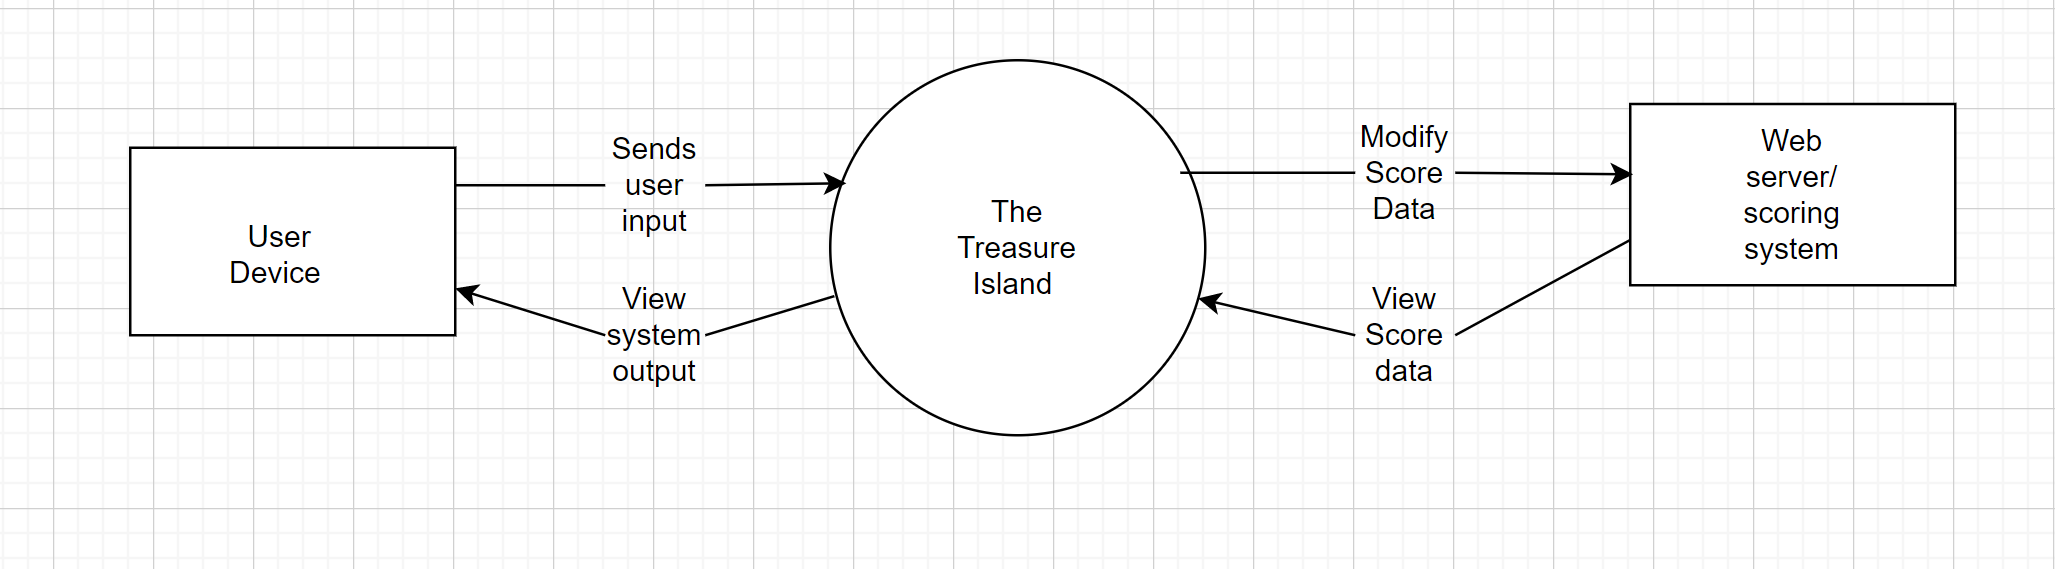
\includegraphics[width=\textwidth]{3A04BlockDiagram.png}

%End-----------------------------------------------------------------------------------------------------------------------------------------------------------------------

\subsection{Product Functions}
\label{sub:product_functions}
% Begin SubSection
% End SubSection

%Start-------------------------------------------------------------------------------------------------------------------------------------------
\subsubsection{Summary of overall product functionality}
The system's major functionality is centralized around the user interacting with the system and participating in the various mini-parts of the system. These aforementioned mini-parts of the system are executed through various mini-games. The game begins by displaying a graphic of a treasure map with a starting point (where the game begins) and an ending point marked as an X (the end of the game), as an innovative feature based on previous playing history the game will predict who is most likely to win. The starting and ending points are separated by 5 individual islands in between, in order to reach the treasure at the end point users must visit each of the islands. Each of these islands is representative of a mini-part/mini-game where the user is required to complete the mini-game in order to advance to the next island and eventually fulfill the main object of the game: get to the treasure. Prior to executing the mini-game on the island, the users will be given a tutorial on how to complete the mini-part/game. Once the user has successfully completed the mini-part/game they will be awarded points (based on score or related scoring metrics) and will advance to the next island (system will display that user has advanced to the next island). Eventually a user will reach the end fulfill the main goal of the game: getting the treasure.

\subsubsection{List of functions:}
\begin{enumerate}[a)]
\item The Treasure Island is a game designed to facilitate friendly competition between loved ones. It will provide different games to collect points and compete.
\item When each mini game is completed, winner of the mini game will progress to the next stage (island) to get closer to the treasure island.
\item The Treasure Island will provide 5 mini-games to the user and make the competition with friends more fair than other games which only relies on skills to be successful in that specific game.
\item In The Treasure Island, users will be rewarded to being good at multiple games.
Users will be able to see their scores and their ranks in a scoreboard to compare their scores with other players.
\item The Treasure Island will provide a map-like \textbf{GUI} to show which stage (island) they are in the game.
\item Users will have access to settings menu in which they can control the sound settings and they can also change/give names to their characters rather than their default names: Player1, Player2.
\item The Treasure Island will provide tutorials for each mini game and the overall game to teach the game rules to the user.
\textcolor{red}{
\item As an innovative feature The Treasure Island will predict and show which user will mostly likely to win the game before the game starts based on several criteria such as high score table, match history etc.
}
\end{enumerate}


%End----------------------------------------------------------------------------------------------------------------------------------------------

\subsection{User Characteristics}
\label{sub:user_characteristics}
% Begin SubSection
The intended users of The Treasure Island are young kids from the ages of 6 - 12, however this product can be used by anyone (teenagers, adults, etc) outside of this range. It is assumed that users of the product have a basic understanding of written English at an elementary proficiency level. The intended user is assumed to have the ability to see and the ability to touch in order to see the visuals of the game as well as interact with the system to provide input. The users are expected to have minimal technical experience, it is assumed they know the basic operations of their device (powering it on, and selecting and launching applications). No other knowledge or experience is expected from the end user.
%End----------------------------------------------------------------------------------------------------------------------------------------------


\subsection{Constraints}
\label{sub:constraints}
\begin{enumerate}[a)]
	\item The system must abide by all Canadian laws.
	\item The system must abide by \textbf{ESRB} E for Everyone rating requirements to make the game suitable for intended users and everyone in the general public.
\end{enumerate}


\subsection{Assumptions and Dependencies}
\label{sub:assumptions_and_dependencies}
% Begin SubSection
% End SubSection

%start--------------------------------------------------------------------------------------------------------------

\begin{enumerate}[a)]
	\item Assumptions
	\begin{itemize}
		\item The user's PC will have the \textbf{minimum system requirements}, but it is advised to use the \textbf{recommended system requirements} to run the game.
		\item The user has a basic understanding/ability of how to use a PC.
		\item The user has at least elementary proficiency in reading English.
	\end{itemize}
	\item Dependencies
	\begin{itemize}
		\item The system's performance is dependent on the speed and quality of the user's hardware specifications and operations systems overhead.
	\end{itemize}
\end{enumerate}

%end--------------------------------------------------------------------------------------------------------------

\subsection{Apportioning of Requirements}
\label{sub:apportioning_of_requirements}
% Begin SubSection
\begin{enumerate}[a)]
	\item Identify requirements that may be delayed until future versions of the system
	\begin{itemize}
	    \item The system shall support more than two players in the multiplayer mode.
	    \item The system shall support more than 5 mini-games. 
	    \item The system shall allow randomization of which mini-game is played at each island. 
    \end{itemize}
\end{enumerate}
% End SubSection

% End Section

\section{Use Case Diagram}
\label{sec:use_case_diagram}
% Begin Section
This section provides a use case diagram for The Treasure Island.\\

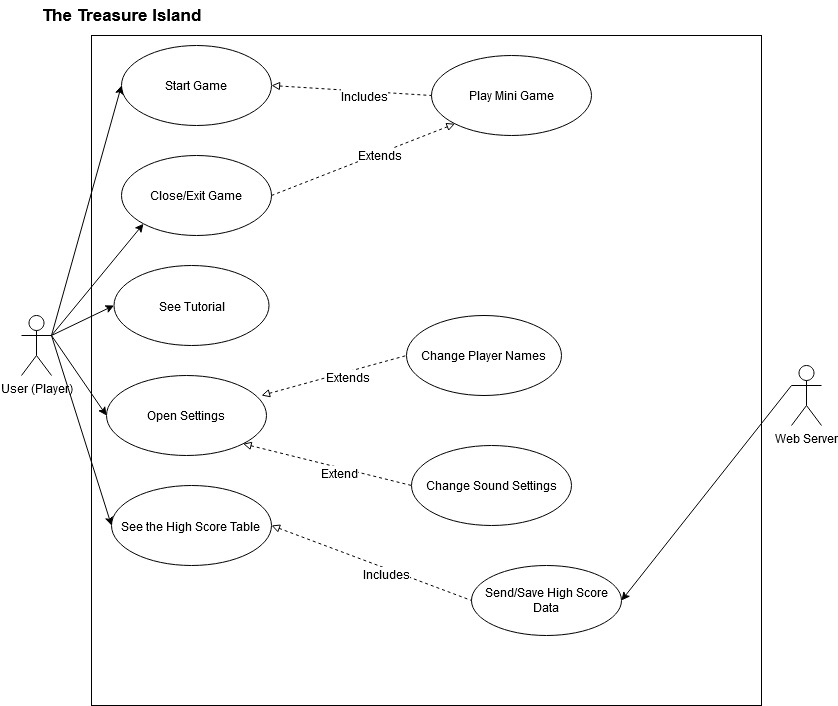
\includegraphics[width=\textwidth]{3A04UsecaseDiagram.jpg}\\\\

%Start-------------------------------------------------------------------------------------------------------------------
Assumption: \textit{All the use cases assume that The Treasure Island game is already open/launched by the user. The user is in the main page/menu of the game to possibly perform the use cases.}

\begin{enumerate}[a)]
    \item Start Game Use Case: User will click on the "Start Game" button to start a new game. After the user starts the game, first mini game will automatically start and Start Game use case is including the Play Game use case because of it.
    \item Close/Exit Game Use Case: If the user is in the main menu of The Treasure Island, user can exit The Treasure Island. If the user is playing a mini game, with the extends relations from the Play Mini Game use case, player can close the current game and return back to The Treasure Island main page.
    \item See Tutorial Use Case: User will click on the "Tutorial" button and will be able to see the rules for The Treasure Island and see the rules and how to play for each mini game as well.
    \item Open Settings Use Case: User can click on the "Settings" button and will be able to see the current settings. Additionally, if the user wants to change the settings, with the extends relations to Change Player Names and Change Sound Settings use cases, user can rename the default names: Player1, Player2; and can change the sound settings.
    \item See the High Scores Table use case: User can click on the "See High Scores" button and, with the includes relationship to the Send/Save High Score Data use case, will see the top ten high scores achieved by any user in the game.
    \item Send/Save High Score Data: When the user scores a high score which is higher than one or more of the users in the high score table, web server will save the user's score to the server. Also, whenever the user request to see high score table, web server will send the high score data to the user's machine.
\end{enumerate}


%End----------------------------------------------------------------------------------------------------------------------

% End Section

\section{Functional Requirements}
\label{sec:functional_requirements}
% Begin Section

%Start------------------------------------------------------------------------------------------------------------------------------------------------------

\begin{enumerate}[{BE}1.]
	\item User starts a new game.
	\begin{enumerate}[{VP1}.1]
		\item User (Player)
			\begin{enumerate}
				\item User shall be able to start a new game from the main menu of The Treasure Island.
				\item User shall be able to choose single or multiplayer mode.
			\end{enumerate}
		\item Security
			\begin{enumerate}
				\item Void
			\end{enumerate}
		\item Legal (\textbf{ESRB})
			\begin{enumerate}
				\item Void
			\end{enumerate}
	\end{enumerate}
	\item User opens tutorial page to learn how the game works.
	\begin{enumerate}[{VP2}.1]
		\item User (Player)
			\begin{enumerate}
				\item User shall be able to see a tutorial to learn about how The Treasure Island can be played.
				\item User shall be able to see tutorials for each mini game to learn how each mini game works.
			\end{enumerate}
		\item Security
			\begin{enumerate}
				\item Void
			\end{enumerate}
		\item Legal (\textbf{ESRB})
			\begin{enumerate}
				\item Tutorials shall not contain any content which will violate \textbf{ESRB} Everyone rating requirements.
			\end{enumerate}
	\end{enumerate}
	\item Request/Save the ten highest scores from/to web server.
	\begin{enumerate}[{VP3}.1]
		\item User (Player)
			\begin{enumerate}
				\item User's score shall be saved both locally and to the web server if the score is in the top ten highest scores.
				\item User shall be able to see high scores from the main page of The Treasure Island.
			\end{enumerate}
		\item Security
			\begin{enumerate}
				\item User shall not receive any malicious data from the web server.
				\item User's data shall not be intercepted when saving or checking the high scores.
			\end{enumerate}
		\item Legal (\textbf{ESRB})
			\begin{enumerate}
				\item User shall not receive any content which will violate \textbf{ESRB} Everyone rating requirements.
				\item User data shall not be shared with any 3rd party other than the web server. 
			\end{enumerate}
	\end{enumerate}
	\item Request to quit from the game.
	\begin{enumerate}[{VP4}.1]
		\item User (Player)
			\begin{enumerate}
				\item User shall be able to quit the game whenever they want without any penalty to their previous scores.
			\end{enumerate}
		\item Security
			\begin{enumerate}
				\item Void
			\end{enumerate}
		\item Legal (\textbf{ESRB})
			\begin{enumerate}
				\item Void
			\end{enumerate}
	\end{enumerate}
	\item User sees/changes settings.
	\begin{enumerate}[{VP5}.1]
		\item User (Player)
			\begin{enumerate}
				\item User shall be able to see and change the sound setting of the game, before or during the game. 
				\item User shall be able to see and change the player name settings before the game starts, but not during the game to avoid confusions in high score table.
				\item If users mute the game no sound will play.
			\end{enumerate}
		\item Security
			\begin{enumerate}
				\item Void
			\end{enumerate}
		\item Legal (\textbf{ESRB})
			\begin{enumerate}
				\item Void
			\end{enumerate}
	\end{enumerate}
\end{enumerate}


%End------------------------------------------------------------------------------------------------------------------------------------------------------

% End Section

\section{Non-Functional Requirements}
\label{sec:non-functional_requirements}
% Begin Section
\subsection{Look and Feel Requirements}
\label{sub:look_and_feel_requirements}
% Begin SubSection

\subsubsection{Appearance Requirements}
\label{ssub:appearance_requirements}
% Begin SubSubSection

\begin{enumerate}[{LF}1. ]
    \item The game should have a starting page that can interact with the player.
    \item The interface shall highlight important areas with different colours.
    \item The images and font size in The Treasure Island should be seen clearly by players.
\end{enumerate}

% End SubSubSection

\subsubsection{Style Requirements}
\label{ssub:style_requirements}
% Begin SubSubSection

\begin{enumerate}[{LF}1. ]
    \item The Treasure Island shall have an appropriate style for target users.
	\item The Treasure Island will bring players some entertainment and provide them excellent and exciting gaming experience.
\end{enumerate}

% End SubSubSection

% End SubSection

\subsection{Usability and Humanity Requirements}
\label{sub:usability_and_humanity_requirements}
% Begin SubSection

\subsubsection{Ease of Use Requirements}
\label{ssub:ease_of_use_requirements}
% Begin SubSubSection

\begin{enumerate}[{UH}1. ]
	\item Each mini game should have a help page on which rules and instructions of that mini game should be shown.
	\item User interface will be clear and simple.
\end{enumerate}

% End SubSubSection

\subsubsection{Personalization and Internationalization Requirements}
\label{ssub:personalization_and_internationalization_requirements}
% Begin SubSubSection

\begin{enumerate}[{UH}1. ]
	\item The game will have a setting page so that players can adjust the volume of the background music and can rename the players rather than their default names: Player1, Player2.
\end{enumerate}

% End SubSubSection

\subsubsection{Learning Requirements}
\label{ssub:learning_requirements}
% Begin SubSubSection

\begin{enumerate}[{UH}1. ]
	\item The help page of each mini-game should have rules that will explain how that mini game works.
\end{enumerate}

% End SubSubSection

\subsubsection{Understandability and Politeness Requirements}
\label{ssub:understandability_and_politeness_requirements}
% Begin SubSubSection

\begin{enumerate}[{UH}1. ]
	\item All text in The Treasure Island will be in Canadian English.
	\item All text in The Treasure Island will not show impolite, discriminational words to any gender, religion, human race.
\end{enumerate}

% End SubSubSection

\subsubsection{Accessibility Requirements}
\label{ssub:accessibility_requirements}
% Begin SubSubSection
\begin{enumerate}[{UH}1. ]
	\item Void
\end{enumerate}
% End SubSubSection

% End SubSection

\subsection{Performance Requirements}
\label{sub:performance_requirements}
% Begin SubSection

\subsubsection{Speed and Latency Requirements}
\label{ssub:speed_and_latency_requirements}
% Begin SubSubSection
\begin{enumerate}[{PR}1. ]
	\item The response time should be less than 30ms for offline parts of the game.
	\item The response time for high scores table will depend on the web server but shall not exceed 10 seconds.
\end{enumerate}

% End SubSubSection

\subsubsection{Safety-Critical Requirements}
\label{ssub:safety_critical_requirements}
% Begin SubSubSection

\begin{enumerate}[{PR}1. ]
	\item The Treasure Island will not transmit any malicious code or program to user's computer.
	\item The Treasure Island will not disclose any user data and personal information.
\end{enumerate}

% End SubSubSection

\subsubsection{Precision or Accuracy Requirements}
\label{ssub:precision_or_accuracy_requirements}
% Begin SubSubSection

\begin{enumerate}[{PR}1. ]
	\item The Treasure Island point system will be accurate to 2 decimal places.
	\item The timer in the software will be accurate to milliseconds.
\end{enumerate}

% End SubSubSection

\subsubsection{Reliability and Availability Requirements}
\label{ssub:reliability_and_availability_requirements}
% Begin SubSubSection

\begin{enumerate}[{PR}1. ]
	\item The game should be accessible and available to the users once they download it.
	\item The game shall exhibit an availability of no less than 95\%.
	\item The game can be played without internet with the exception of global high score server.
\end{enumerate}
% End SubSubSection


\subsubsection{Robustness or Fault-Tolerance Requirements}
\label{ssub:robustness_or_fault_tolerance_requirements}
% Begin SubSubSection

\begin{enumerate}[{PR}1. ]
	\item The system shall not crash when the user has no internet connection but requests to check the high scores from the web server. Instead, The Treasure Island shall show an error message to inform the user and only show the locally stored user's highest score.
\end{enumerate}

% End SubSubSection

\subsubsection{Capacity Requirements}
\label{ssub:capacity_requirements}
% Begin SubSubSection

\begin{enumerate}[{PR}1. ]
	\item The system shall be able to respond to at least 2 players at the same time.
	\item The game will have \textbf{minimum system requirements} to be played without any performance issues.
\end{enumerate}
% End SubSubSection


\subsubsection{Scalability or Extensibility Requirements}
\label{ssub:scalability_or_extensibility_requirements}
% Begin SubSubSection

\begin{enumerate}[{PR}1. ]
	\item The system should be able to allow more than two players.
\end{enumerate}

% End SubSubSection

\subsubsection{Longevity Requirements}
\label{ssub:longevity_requirements}
% Begin SubSubSection
% This section means what is the life expectancy of the software.
\begin{enumerate}[{PR}1. ]
	\item Void
\end{enumerate}

% End SubSubSection

% End SubSection

\subsection{Operational and Environmental Requirements}
\label{sub:operational_and_environmental_requirements}
% Begin SubSection

\subsubsection{Expected Physical Environment}
\label{ssub:expected_physical_environment}
% Begin SubSubSection

\begin{enumerate}[{OE}1. ]
	\item The Treasure Island should be able to run in any physical environment that can be supported by PC.
\end{enumerate}

% End SubSubSection

\subsubsection{Requirements for Interfacing with Adjacent Systems}
\label{ssub:requirements_for_interfacing_with_adjacent_systems}
% Begin SubSubSection

\begin{enumerate}[{OE}1. ]
    \item The Treasure Island will interface with the PC operating systems to allow installing, uninstalling, updating the game and saving the user scores locally.
\end{enumerate}

% End SubSubSection

\subsubsection{Productization Requirements}
\label{ssub:productization_requirements}
% Begin SubSubSection
\begin{enumerate}[{OE}1. ]
	\item The product shall be free.
\end{enumerate}
% End SubSubSection

\subsubsection{Release Requirements}
\label{ssub:release_requirements}
% Begin SubSubSection

\begin{enumerate}[{OE}1. ]
	\item The Treasure Island's binary code (executable files) will be hosted on a website and users can download it from the website.
	\item For each update, users will need to download the new version of The Treasure Island from the release website.
\end{enumerate}

% End SubSubSection

% End SubSection

\subsection{Maintainability and Support Requirements}
\label{sub:maintainability_and_support_requirements}
% Begin SubSection

\subsubsection{Maintenance Requirements}
\label{ssub:maintenance_requirements}
% Begin SubSubSection

\begin{enumerate}[{MS}1. ]
	\item Each class and internal function should be documented and commented to allow others to understand the program easily.
	\item Any changes to functions and methods should be documented.
\end{enumerate}
% End SubSubSection


\subsubsection{Supportability Requirements}
\label{ssub:supportability_requirements}
% Begin SubSubSection

\begin{enumerate}[{MS}1. ]
	\item The software shall be able to run on at least 95\% of computers which meets the \textbf{minimum system requirements}.
\end{enumerate}

% End SubSubSection

\subsubsection{Adaptability Requirements}
\label{ssub:adaptability_requirements}
% Begin SubSubSection

\begin{enumerate}[{MS}1. ]
	\item Void
\end{enumerate}

% End SubSubSection

% End SubSection

\subsection{Security Requirements}
\label{sub:security_requirements}
% Begin SubSection

\subsubsection{Access Requirements}
\label{ssub:access_requirements}
% Begin SubSubSection

\begin{enumerate}[{SR}1. ]
    \item Users can access any mini games without difficulty in The Treasure Island's main page.
\end{enumerate}

% End SubSubSection


\subsubsection{Integrity Requirements}
\label{ssub:integrity_requirements}
% Begin SubSubSection
\begin{enumerate}[{SR}1. ]
	\item High scores in the web server shall not be tempered with to maintain the integrity of the high score data.
\end{enumerate}
% End SubSubSection

\subsubsection{Privacy Requirements}
\label{ssub:privacy_requirements}
% Begin SubSubSection

\begin{enumerate}[{SR}1. ]
	\item User data will not be shared with any 3rd party unless it is required for the 3rd party services (e.g. database to keep user scores) to work. In the later case, users will be informed and their consent will be required to share the data.
\end{enumerate}

% End SubSubSection

\subsubsection{Audit Requirements}
\label{ssub:audit_requirements}
% Begin SubSubSection

\begin{enumerate}[{SR}1. ]
	\item Void
\end{enumerate}

% End SubSubSection

\subsubsection{Immunity Requirements}
\label{ssub:immunity_requirements}
% Begin SubSubSection

\begin{enumerate}[{SR}1. ]
	\item Void
\end{enumerate}

% End SubSubSection

% End SubSection

\subsection{Cultural and Political Requirements}
\label{sub:cultural_and_political_requirements}
% Begin SubSection

\subsubsection{Cultural Requirements}
\label{ssub:cultural_requirements}
% Begin SubSubSection

\begin{enumerate}[{CP}1. ]
	\item The software will not include any symbols, images or text that may be considered as offensive or rude to users. 
\end{enumerate}

% End SubSubSection

\subsubsection{Political Requirements}
\label{ssub:political_requirements}
% Begin SubSubSection
\begin{enumerate}[{CP}1. ]
	\item The system must meet the standards and requirements set by the management (Dr.Khedri, Thien Trandinh, and Andrew Le Clair)
\end{enumerate}
% End SubSubSection

% End SubSection

\subsection{Legal Requirements}
\label{sub:legal_requirements}
% Begin SubSection

\subsubsection{Compliance Requirements}
\label{ssub:compliance_requirements}
% Begin SubSubSection
\begin{enumerate}[{LR}1. ]
	\item The system shall function within the jurisdiction of Canada.
\end{enumerate}
% End SubSubSection

\subsubsection{Standards Requirements}
\label{ssub:standards_requirements}
% Begin SubSubSection
\begin{enumerate}[{LR}1. ]
	\item The system must meet the Everyone rating requirements set by \textbf{ESRB}.
\end{enumerate}
% End SubSubSection

% End SubSection

% End Section

\appendix
\section{Division of Labour}
\label{sec:division_of_labour}
% Begin Section
The following below includes a description of the division of labour for this document. \\

\noindent\textbf{Mohinder Kallay} \\
Made contributions to all subsections of section 1 and section 2. \\
\textbf{Abdullah Abdul Maksoud} \\ 
Contributed to all subsections of section 1 except subsection 1.2, contributed to all subsections of section 2 except subsection 2.1, 2.2, and contributed to sections 3, 4, and 5\\
\textbf{Namik Karaata} \\ 
Made contributions to every subsection in section 1 except subsection 1.5, made contributions to every subsection in section 2 except subsection 2.6. Contributed to section 3 and 4. Contributed to more than 35\% of the section 5.\\
\textbf{Gengyun Wang} \\
Made contributions to some subsections of section 4 and 5. \\
\textbf{Junhong Chen} \\
Contributed to some subsections of section 4 and section 5. \\

	\noindent\begin{tabular}{ll}\\
	M.K & February 5, 2021 \\
	\makebox[2.5in]{\hrulefill} & \makebox[2.5in]			{\hrulefill}\\
	Mohinder Kallay & Date\\[8ex]% adds space between the two sets of signatures
	A.A. & February 5, 2021 \\
	\makebox[2.5in]{\hrulefill} & \makebox[2.5in]			{\hrulefill}\\
	Abdullah Abdul Maksoud & Date\\[8ex]
	N.K. & February 5, 2021 \\
	\makebox[2.5in]{\hrulefill} &  \makebox[2.5in]			{\hrulefill}\\
	Namik Karaata & Date\\[8ex]
	G.W & February 5, 2021 \\
	\makebox[2.5in]{\hrulefill} & \makebox[2.5in]			{\hrulefill}\\
	Gengyun Wang & Date\\[8ex]
	J.C & February 5, 2021 \\
	\makebox[2.5in]{\hrulefill} & \makebox[2.5in]			{\hrulefill}\\
	Junhong Chen & Date\\
	\end{tabular}
% End Section

\end{document}
%------------------------------------------------------------------------------